\chapter{Introduction}\label{ch:intro}

Thermoelectric conversion is attractive for distributed power generation, waste heat recovery, and thermal regulation because it uses solid-state modules with no moving parts \citep{bell2008cooling,snyder2008complex}. Yet practical operation often occurs under time-varying heat loads, causing unstable temperature gradients and suboptimal conversion efficiency. This dissertation addresses that transient bottleneck through a materials architecture in which a phase change material is embedded in a \textbf{hierarchical nanoporous PVA scaffold} reinforced with CuS--MoS$_2$ nanofillers.

\section{Research Gap and Problem Statement}
Three gaps motivate this work. First, most thermoelectric optimization studies emphasize static $ZT$ enhancement while neglecting transient thermal buffering \citep{he2017advances}. Second, PCM-integrated thermal management frequently uses metallic or ceramic matrices with limited flexibility and high interfacial mismatch \citep{zhang2020pcmreview}. Third, composite studies can ambiguously attribute scaffold function to fillers. In this dissertation, the scaffold is strictly PVA, CuS--MoS$_2$ only reinforces PVA, and PCM is confined inside PVA porosity.

The governing challenge is maximizing net electrical output under fluctuating thermal sources while minimizing entropy generation and mechanical degradation across cycles.

\section{Objectives}
The main objective is to establish and validate a design framework for PVA/PCM/CuS--MoS$_2$ thermoelectric coupling. Sub-objectives include:
\begin{enumerate}[label=(\roman*)]
    \item formulate coupled transport and phase-change equations,
    \item design hierarchical pore architecture for PCM confinement,
    \item quantify filler-driven transport enhancement without violating scaffold continuity,
    \item evaluate exergy and irreversibility metrics under cycling.
\end{enumerate}

\section{Novelty}
The explicit novelty is the tri-functional separation of roles:
\begin{itemize}
    \item \textbf{PVA:} continuous mechanical scaffold and porous host,
    \item \textbf{PCM:} latent thermal buffer within PVA pores,
    \item \textbf{CuS--MoS$_2$:} reinforcing nanofillers to tune conductivity and interfaces.
\end{itemize}

\begin{equation}\label{eq:intro_power_balance}
\dot{W}_{net}=\int_{A}\left(S\,\Delta T\right)\,\mathrm{d}I-\dot{Q}_{loss},
\end{equation}
where thermal buffering reduces $\dot{Q}_{loss}$ during high-frequency fluctuations.

\begin{figure}[htbp]
\centering
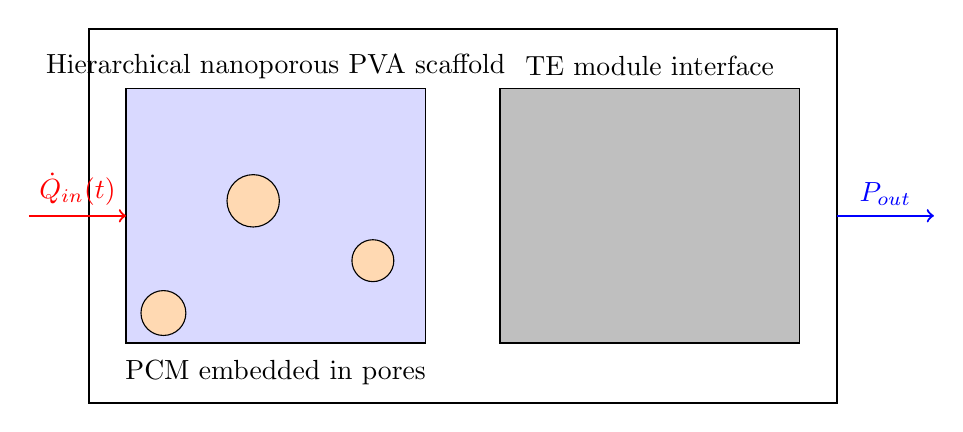
\begin{tikzpicture}[scale=0.95]
\draw[thick] (0,0) rectangle (10,5);
\draw[fill=blue!15] (0.5,0.8) rectangle (4.5,4.2);
\draw[fill=orange!30] (1.0,1.2) circle (0.3);
\draw[fill=orange!30] (2.2,2.7) circle (0.35);
\draw[fill=orange!30] (3.8,1.9) circle (0.28);
\draw[fill=gray!50] (5.5,0.8) rectangle (9.5,4.2);
\node at (2.5,4.5) {Hierarchical nanoporous PVA scaffold};
\node at (2.5,0.4) {PCM embedded in pores};
\node at (7.5,4.5) {TE module interface};
\draw[->,thick,red] (-0.8,2.5) -- (0.5,2.5) node[midway,above] {$\dot{Q}_{in}(t)$};
\draw[->,thick,blue] (10,2.5) -- (11.3,2.5) node[midway,above] {$P_{out}$};
\end{tikzpicture}
\caption{Conceptual architecture: PCM-filled pores within a PVA scaffold reinforced by dispersed CuS--MoS$_2$ fillers adjacent to a thermoelectric module.}
\label{fig:intro_architecture}
\end{figure}

\begin{table}[htbp]
\centering
\caption{Dissertation-level research questions.}
\label{tab:intro_questions}
\begin{tabular}{p{1.2cm}p{11.2cm}}
\toprule
ID & Research Question \\
\midrule
RQ1 & How does PCM confinement in PVA pores alter transient thermal gradients across a TE leg? \\
RQ2 & What CuS--MoS$_2$ loading maximizes effective transport while preserving mechanical integrity? \\
RQ3 & How do entropy generation and exergy efficiency evolve under repeated thermal cycles? \\
\bottomrule
\end{tabular}
\end{table}

\section{Dissertation Organization}
\Cref{ch:lit} reviews prior work; \Cref{ch:te_theory,ch:pcm,ch:pva,ch:cusmos2} establish theory and material foundations; \Cref{ch:multi} presents coupled modeling; \Cref{ch:case,ch:exergy} report performance analyses; \Cref{ch:future,ch:conclusion} discuss implications and contributions.
